\documentclass[12pt]{article}
\usepackage{amsmath,amsfonts,times}
\usepackage{graphicx,color,tikz,pgfplots}
\usepackage[paperwidth=16.1cm,paperheight=8.1cm,lmargin=0in,rmargin=0in,tmargin=0.in,bmargin=0.in]{geometry}
\usepackage{bm}
\usetikzlibrary{arrows,shadings,shapes.arrows,decorations.pathreplacing,calc, positioning}
\usepgfplotslibrary{fillbetween}

\begin{document}

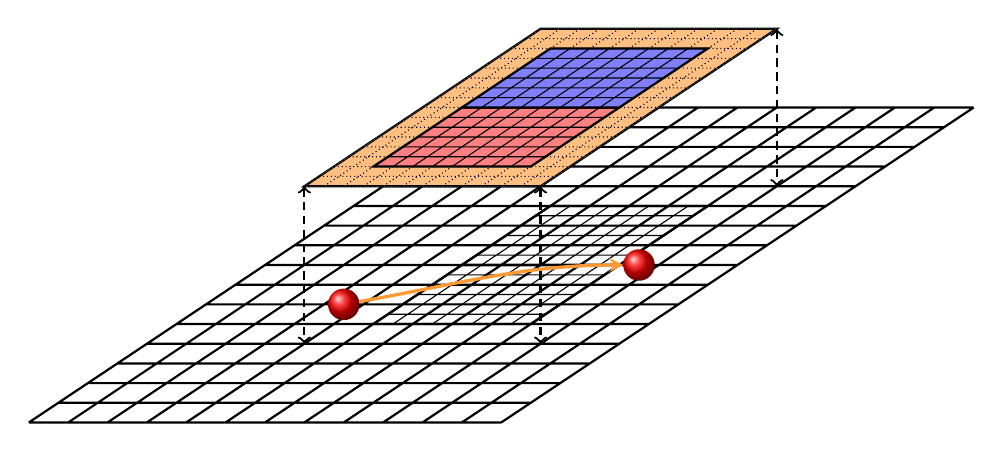
\begin{tikzpicture}[on grid,x=1cm, y=1cm]
  \draw[xslant=1.5, thick] (0,0) grid[xstep=0.5, ystep=0.25] (6,4);

  \begin{scope}[xshift=3.5cm, yshift=1cm]
%    \draw[draw=none, thick, xslant=1.5, fill=white, fill opacity=1.0] (0,0) rectangle(3,2);
%    \draw[densely dotted, fill=white, thin, xslant=1.5] grid[xstep=0.25, ystep=0.125] (3,2);
    
    \draw[solid, draw=black, thick, xslant=1.5] (0.5,0.25) rectangle(2.5,1.0);
    \draw[solid, black, thin, xslant=1.5] (0.5, 0.25) grid[xstep=0.25, ystep=0.125] (2.5,1.0);

   \draw[solid, draw=black, thick, xslant=1.5] (0.5, 1.0) rectangle(2.5,1.75);    
   \draw[solid, black, thin, xslant=1.5]       (0.5, 1.0) grid[xstep=0.25, ystep=0.125] (2.5,1.75);        
   %    \draw[fill=black, thin, xslant=1.5] grid[xstep=0.25, ystep=0.125] (3,2);
  \end{scope}

  \begin{scope}[xshift=3.5cm, yshift=3cm]
    \draw[draw=black, thick, xslant=1.5, fill=orange!50!white, fill opacity=1.0] (0,0) rectangle(3,2);
    \draw[densely dotted, fill=white, thin, xslant=1.5] grid[xstep=0.25, ystep=0.125] (3,2);
    
    \draw[solid, draw=black, thick, xslant=1.5, fill=red!50!white] (0.5,0.25) rectangle(2.5,1.0);
    \draw[solid, black, thin, xslant=1.5] (0.5, 0.25) grid[xstep=0.25, ystep=0.125] (2.5,1.0);

    \draw[solid, draw=black, thick, xslant=1.5, fill=blue!50!white] (0.5, 1.0) rectangle(2.5,1.75);    
    \draw[solid, black, thin, xslant=1.5]       (0.5, 1.0) grid[xstep=0.25, ystep=0.125] (2.5,1.75);        
    
    \draw[thick, <->, densely dashed, black] (0,0) -- ++(0,-2);
    \draw[thick, <->, densely dashed, black] (6,2) -- ++(0,-2);
    \draw[thick, <->, densely dashed, black] (3,0) -- ++(0,-2);        
  \end{scope}

  \begin{scope}[xshift=3.5cm, yshift=1cm]

   
    \shade[ball color = red, opacity=1.0] (0.5,0.5) circle(2mm);
    \shade[ball color = red, opacity=1.0] (4.25,1) circle(2mm);


   %   \node[circle, shading=ball, outer color=red, inner color=white, minimum width=2mm, alias=e2] at (4,1) {};

    \draw[very thick, orange!80!white, -stealth, shorten <= 2mm, shorten >= 2mm] (0.5,0.5) to[out=10, in=180] (4.25,1);   
  \end{scope}  
\end{tikzpicture}

\end{document} 
